\documentclass{scrartcl}
\usepackage{graphicx}
\title{Confusa architecture documentation}
\author{Henrik Austad \& Thomas Zangerl}

\begin{document}

\maketitle
\newpage
\tableofcontents
\newpage

\section{Authentication in Confusa}

Authentication in Confusa is mostly done by calling the simplesamlphp\footnote{http://rnd.feide.no/simplesamlphp} subsystem, which will take care of AuthN and deAuthN by performing the login-redirects and consuming the SAML assertions that are sent by the IdPs.

Most information about the currently logged on user is administered in the Person class, which is just a convenient data store for all information that is received from the IdPs.

Figure \ref{confusa_auth_classes} shows the framework of authentication classes in Confusa. The state in which we want to end is having a fully "decorated" person, i.e. a person that has all attributes that we need to know about her assigned to her member variables. Assuming that we know nothing about the person and a sensitive action in Confusa, which requires such knowledge, is selected, Confusa performs the following steps:

\begin{enumerate}
	\item[1] The AuthHandler picks the right ConfusaAuth-subclass for the current situation. Often that is \verb+ConfusaAuth_IdP+, which handles authN using a WebSSO SAML2 redirect in simplesamlphp to authN the user.
	\item[2] authenticateUser() in the ConfusaAuth-subclass authenticates the user and makes sure to get her attributes. In \verb+ConfusaAuth_IdP+, the user is redirected to the initSSO page of simplesamlphp which will take care of the rest.
	\item[3] When Confusa is then opened again, because simplesamlphp relayed the user back to the site that initiated the request, the attributes are assigned to the person using the decoratePerson() method in \verb+Confusa_Auth+.
	\item[4] Different IdPs may send different attribute names for the same attributes. For instance, the name of the user may be send as "cn" \verb+=>+ "John Doe" or "displayName" \verb+=>+ "John Doe" or "name" \verb+=>+ "John Doe". Therefore, we must keep a mapping of the different attribute keys of the NRENs and subscribers to the attribute keys we need. That mapping is defined in the admin menu and kept in the database. Upon decoration of the person the mapping is looked up to assign the right attribute values to the right attributes. For that, getMap() in AuthHandler is called. See figure \ref{confusa_attr_mapping} for schematics of the process.
	\item[5] With the right attribute keys, the attribute values can be retrieved and ConfusaAuth can decorate the person, which is now authenticated and generously providing user information to other components of Confusa.
\end{enumerate}

\begin{figure}\label{confusa_auth_classes}
\begin{center}
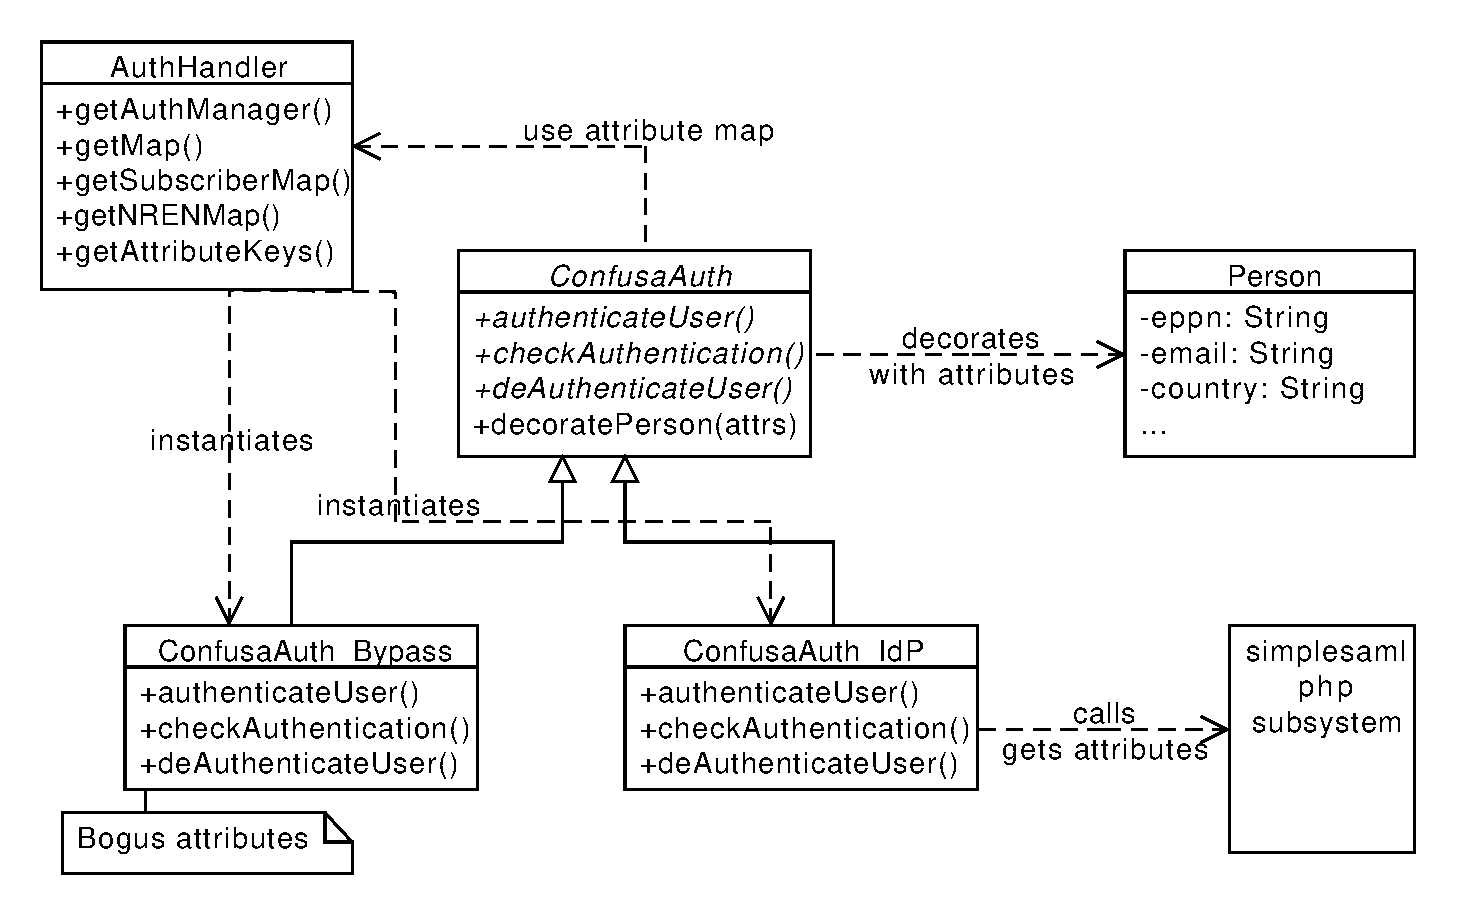
\includegraphics[width=\textwidth]{auth_classes}
\caption{The Confusa Auth classes}
\end{center}
\end{figure}

\begin{figure}\label{confusa_attr_mapping}
\begin{center}
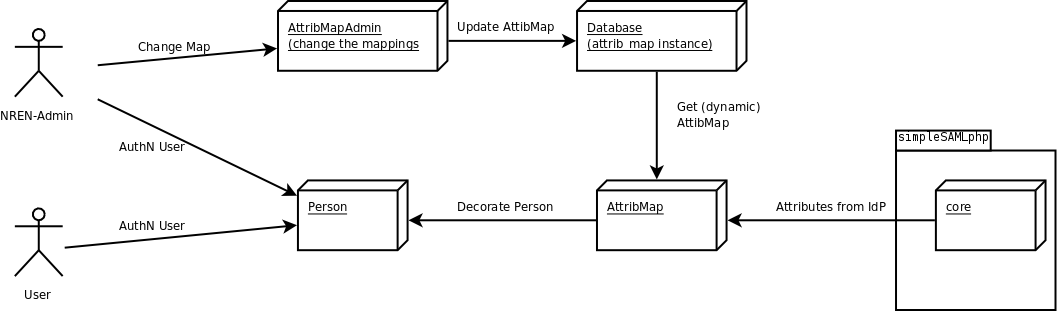
\includegraphics[width=\textwidth]{AttribMap.png}
\caption{Confusa attribute mapping process}
\end{center}
\end{figure}

\textbf{deAuthenticating} (logging out) the user is even simpler.

\begin{enumerate}
	\item[1] Confusa forgets all attributes of the user by unsetting the fields in Person.
	\item[2] For IdPs not supporting SingleLogout (SLO), Confusa calls a simplesamlphp logout procedure that calls registered logout hooks, i.e. attributes that were sent by the IdPs for logging out.
	\item[3] For those IdPs that support (SLO), Confusa just redirects to simplesamlphp's initSLO page. Otherwise, Confusa has to find a logout address in the attributes sent by the IdP
\end{enumerate}

\section{Certificate request signing in Confusa}

\subsection{Confusa modes}

Confusa can sign certificates in two modes

\begin{itemize}
	\item Using its own certificate and key (\emph{standalone})
	\item Using the HTTP POST API of Comodo (\emph{online})
\end{itemize}

Depending on the mode the behaviour is slightly different. For standalone-mode, an \verb+auth_key+, which is a pubkey-hash, is the main identifier of the certificate, while in online-mode, an \verb+order-number+ serves as Confusa's ID for the certificate.

\begin{figure}\label{csr_sign_online}
\begin{center}
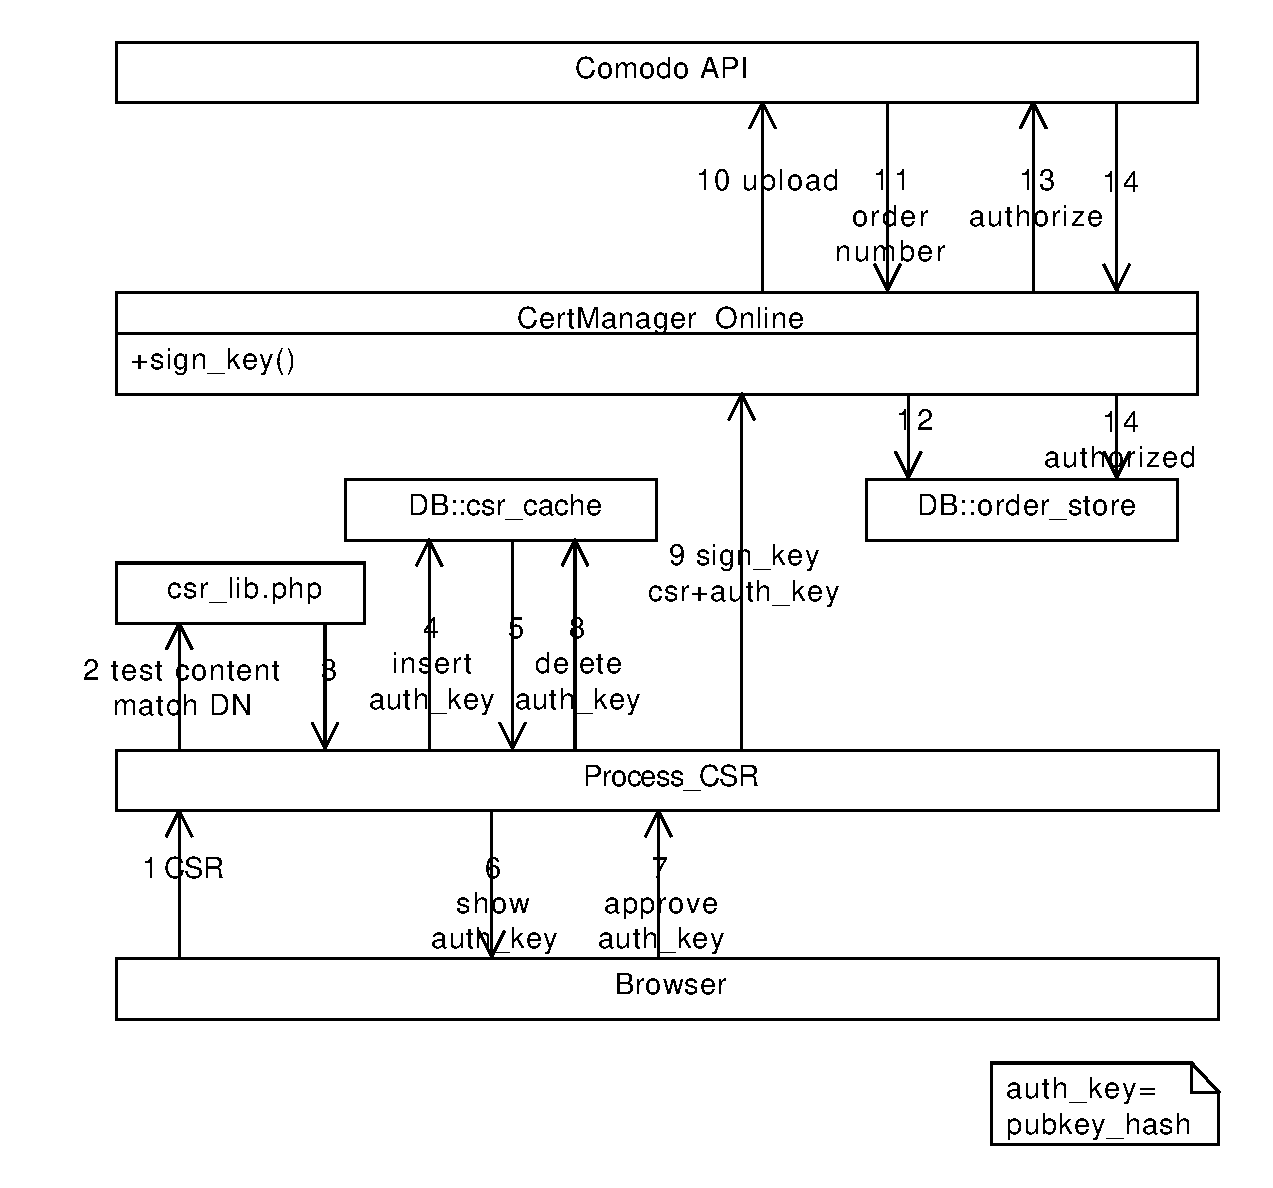
\includegraphics[width=\textwidth]{cm_online_flow}
\end{center}
\end{figure}

\begin{figure}\label{csr_sign_standalone}
\begin{center}
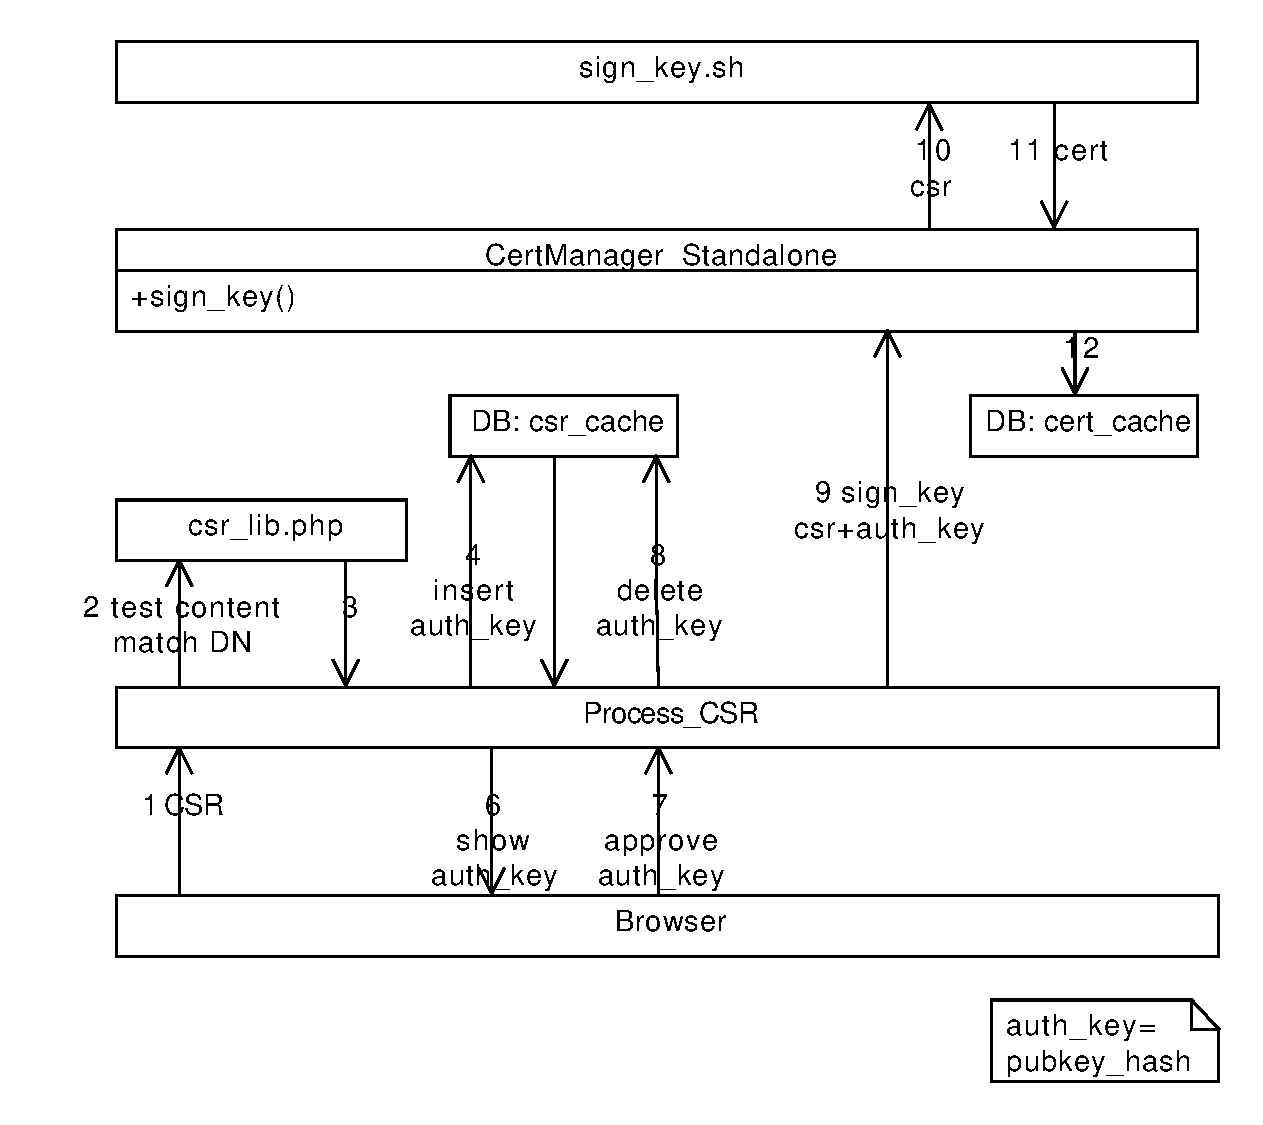
\includegraphics[width=\textwidth]{cm_standalone_flow}
\caption{CSR signing flow in Confusa's standalone configuration}
\end{center}
\end{figure}

\subsection{Certificate signing in online-mode}

The flow of certificate signing in online mode is shown in figure \ref{csr_sign_online}. The following steps are followed by Confusa:

\begin{enumerate}
	\item[1] The user uploads a CSR using her browser
	\item[2] An \verb+auth_key+ is computed, which is the first 16 characters of the pubkey-hash.
	\item[3] \verb+Process_CSR+ passes the CSR to \verb+csr_lib.php+ to check for well-formedness and known-problems (is the pubkey already known? is the RSA algorithm used? does the key-length match the configuration? was the vulnerable Debian openssl software used for generating the CSR?).
	\item[4] If everything is okay in steps 1 to 3, then Confusa inserts the CSR into the DB where it will be stored for some time (default: 10 minutes).
	\item[5] Within that timeframe, the user has the chance to approve the CSR for signing. If the user approves the request, it will be deleted from the DB and passed to \verb+CertManager_Online+
	\item[6] \verb+CertManager_Online+ takes the request and uploads it using a HTTP POST request to the Comodo API. The Comodo API returns an order-number.
	\item[7] \verb+CertManager_Online+ inserts the \verb+auth_key+, order-number and other certificate releated information into the \verb+order_store+ table in the database
	\item[8] In the next step, the Comodo-API is contacted to authorize the signing request.
	\item[9] If the request was successfully authorized, this is reflected in the DB. Now, the certficate is processed by Comodo and will appear in the download-list later on.
\end{enumerate}

\subsection{Certificate signing in standalone-mode}

Figure \ref{csr_sign_standalone} shows the standalone-signing mode, which is quite similar to the online-signing mode. For standalone-signing to work, CA-certificates must be present in the \verb+cert_handle/+ directory of Confusa and certain files such as ca.db.serial must be writeable by the webserver-user.
Certificate signing in standalone works as follows (steps 1 and 2 are the same as in online mode):

\begin{enumerate}
	\item[3] Is the same as in online mode, but additionally it is checked if the subject-DN of the CSR matches the attributes that were received from the identity provider. It is only thus that Confusa can ensure that the user only issues certificates to herself.
	\item[4] If everything is okay in steps 1 to 3, then Confusa inserts the CSR into the DB where it will be stored for some time (default: 10 minutes).
	\item[5] Within that timeframe, the user has the chance to approve the CSR for signing. If the user approves the request, it will be deleted from the DB and passed to \verb+CertManager_Standalone+
	\item[6] \verb+CertManager_Standalone+ passes the CSR to a shell script within the \verb+cert_handle/+ directory of Confusa, which will call openssl and thus sign the CSR with the installed CA certificates. The signed certificate is returned to \verb+CertManager_Standalone+.
	\item[7] \verb+CertManager_Standalone+ inserts the certificate into the \verb+cert_cache+ table in the DB, where it can be picked up for download later on.
\end{enumerate}

\subsection{Certificate signing for browser requests}

\emph{Note: Browser requests currently work only in online mode.}

For browser requests, certificate signing works a bit different. First, browsers are a quite inhomogenous kind: they don't have an uniform crypto API, nor do they all support the semi-official \verb+<keygen>+ tag. Different versions of IE generate certificate requests in \verb+PKCS#10+ format, Firefox's crypto-API in CMRF-format and the \verb+<keygen>+ tag outputs SPKAC (Signed Public Key And Challenge), a Netscape format that is, however, supported by OpenSSL.

We use

\begin{itemize}
	\item XEnroll.dll for Internet Explorer on Windows XP and Server 2003
	\item CertEnroll.dll for Internet Explorer on Windows Vista, Server 2008 and Windows 7
	\item \verb+<keygen>+ for all other browsers
\end{itemize}

Initially we used Firefox's Crypto-API for Firefox, but because of the bad support of the CRMF-standard that was dropped in favour of universal use of the \verb+<keygen>+ tag. JavaScript is needed for all browsers, even though \verb+<keygen>+ could work without, to keep the programmatic part as simple as possible and - more important - to have the same user flow for all browsers. And if some crypto API will appear for other browsers as well, it will be easier to hook into that.

Figures \ref{fig_browser_process} and \ref{fig_browser_deploy} illustrate processing and deployment of certificates in the browser.

When processing a browser request,

\begin{enumerate}
	\item[1] The browser generates a CSR, in \verb+PKCS#10+ or SPKAC and a private key. The private key goes into the browser's keystore. The CSR is submitted in a POST message to \verb+Process_CSR+.
	\item[2] \verb+Process_CSR+ calls signBrowserCSR, along with the user-agent that made the request in \verb+CertManager_Online+.
	\item[3] The request is sent to Comodo using the HTTP POST API, a order number is returned.
	\item[4] The order-number is passed through all components down to the JavaScript, which will periodically poll for the status of the order using HTTP GET messages.
	\item[5] Whenever \verb+Process_CSR+ is polled for the status, it will itself query the backend, which will query the Comodo API for the status.
	\item[6] Once processing was successful, a "done" status is pushed down to the JavaScript, which will stop polling and instead use DOM manipulations to show an install-link on the page.
\end{enumerate}

If the user clicks the install-link on the page, or in the download-section, the following happens:

\begin{enumerate}
	\item[1] A HTTP GET message is sent to \verb+Process_CSR+.
	\item[2] \verb+Process_CSR+ queries \verb+CertManager_Online+ for a certificate deployment script for the \verb+order_number+, passing the user agent as a second argument.
	\item[3] \verb+CertManager_Online+ queries the Comodo API for the certificate in the right format, that means dependant on the browser either the full-chain or only the certificate itself and either a certificate or executable JavaScript code for certificate installation.
	\item[4] Once it has the certificate, it either returns it, or wraps it in \verb+<script>+ tags so it can be executed.
	\item[5] The certificate in the right format gets passed down to \verb+Process_CSR+. Dependant on the user agent, it will be passed to \verb+download_certificate+ in \verb+file_download.php+ or passed down to the JavaScript for execution.
\end{enumerate}

\begin{figure}\label{fig_browser_process}
	\begin{center}
	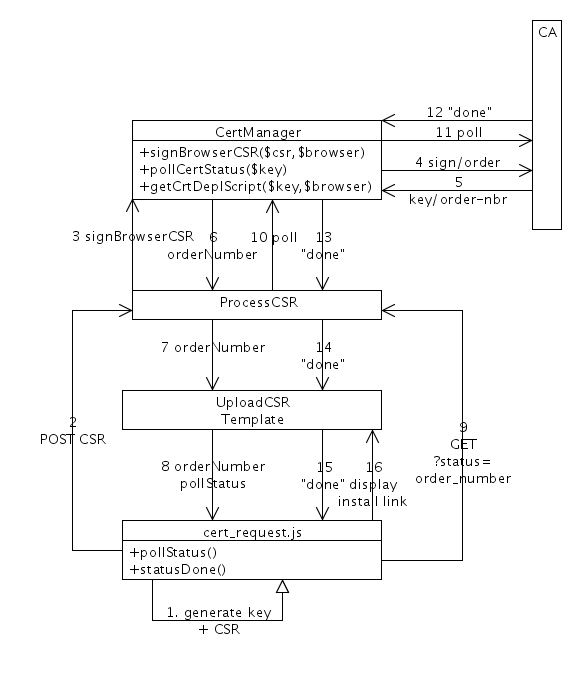
\includegraphics[width=\textwidth]{browser_process_cert}
	\caption{Processing of browser certificate requests}
	\end{center}
\end{figure}

\begin{figure}\label{fig_browser_deploy}
	\begin{center}
		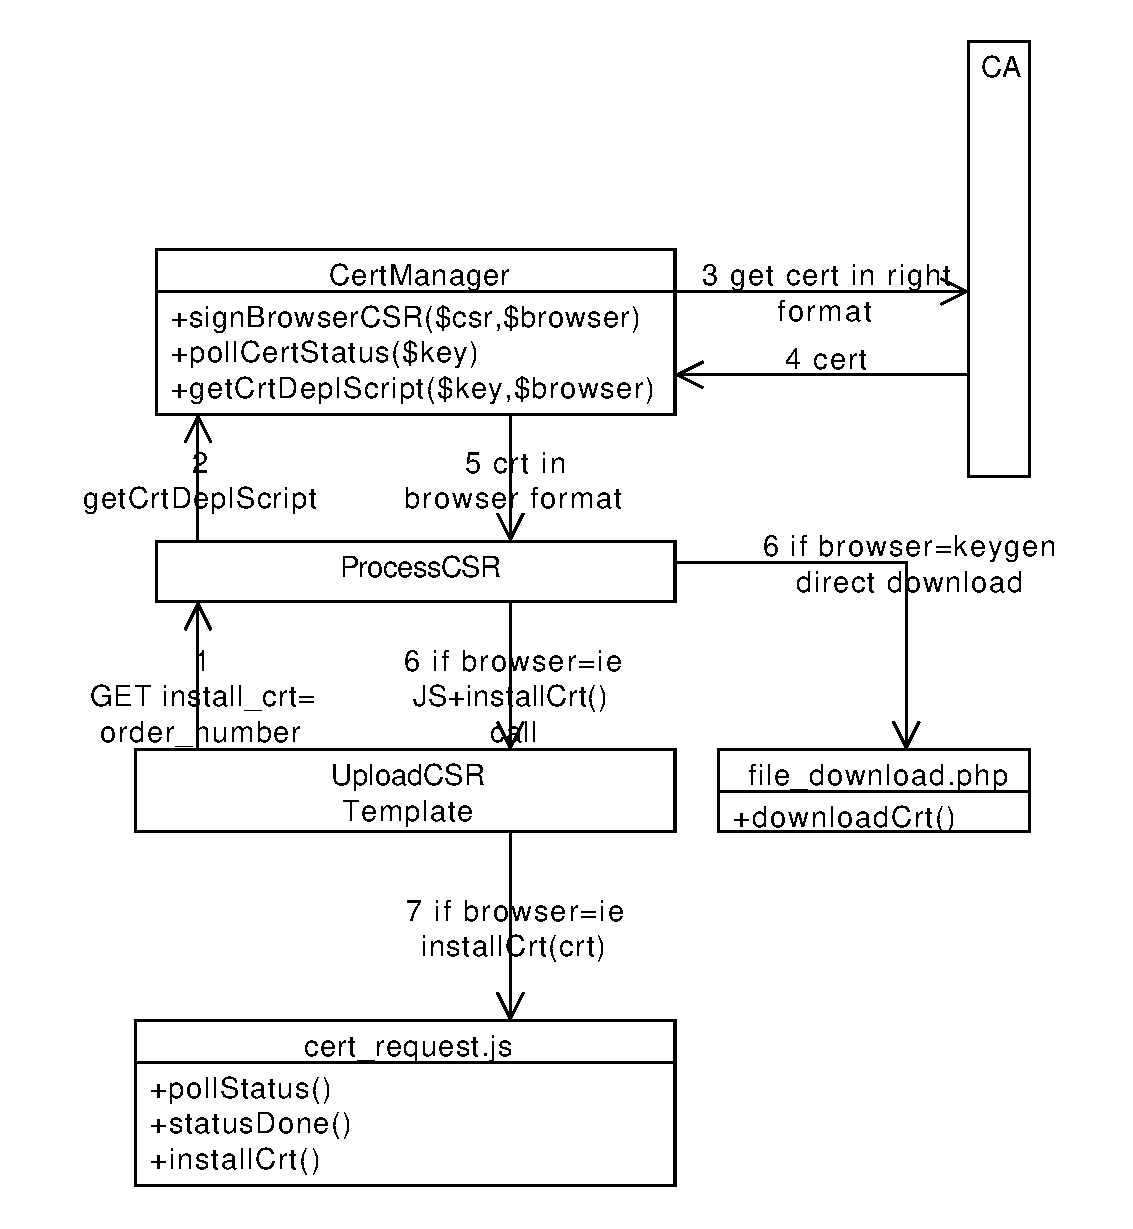
\includegraphics[width=\textwidth]{browser_deploy_cert}
		\caption{Deployment of certificates in browsers}
	\end{center}
\end{figure}

\section{The Framework}

All visible Confusa pages should be embedded in the \verb+Framework+ class, subclassing \verb+ContentPage+. The communication between the \verb+Framework+ and the \verb+ContentPage+ is detailed in figure \ref{fig_seq_fw}.

The framework is roughly responsible for the following things:

\begin{itemize}
	\item Ensure a decorated person object is in place
	\item Initiate user authentication if the content-page is protected (restricted to authN users)
	\item Call \verb+pre_process+, process and \verb+post_process+ on the ContentPage
	\item Render fixed component of Confusa itself (NREN-logo, menu, include NREN-CSS)
	\item Display of notification messages
\end{itemize}

The ContentPage is the superclass for all pages of Confusa showing actual content. The actual content is stored in a Smarty\footnote{http://www.smarty.net/} template. The ContentPage is called by Framework in three phases:

\begin{itemize}
	\item \verb+pre_process:+ Things to be done before the content of the page (template) is shown. E.g. processing of POST parameters, translation of strings on the page.
	\item \verb+process:+ Things to be done when the content of the page is shown, e.g. assigning template variables.
	\item \verb+post_process:+ Things to be done after the page has been displayed. Cleanup...
\end{itemize}

\begin{figure}\label{fig_seq_fw}
	\begin{center}
	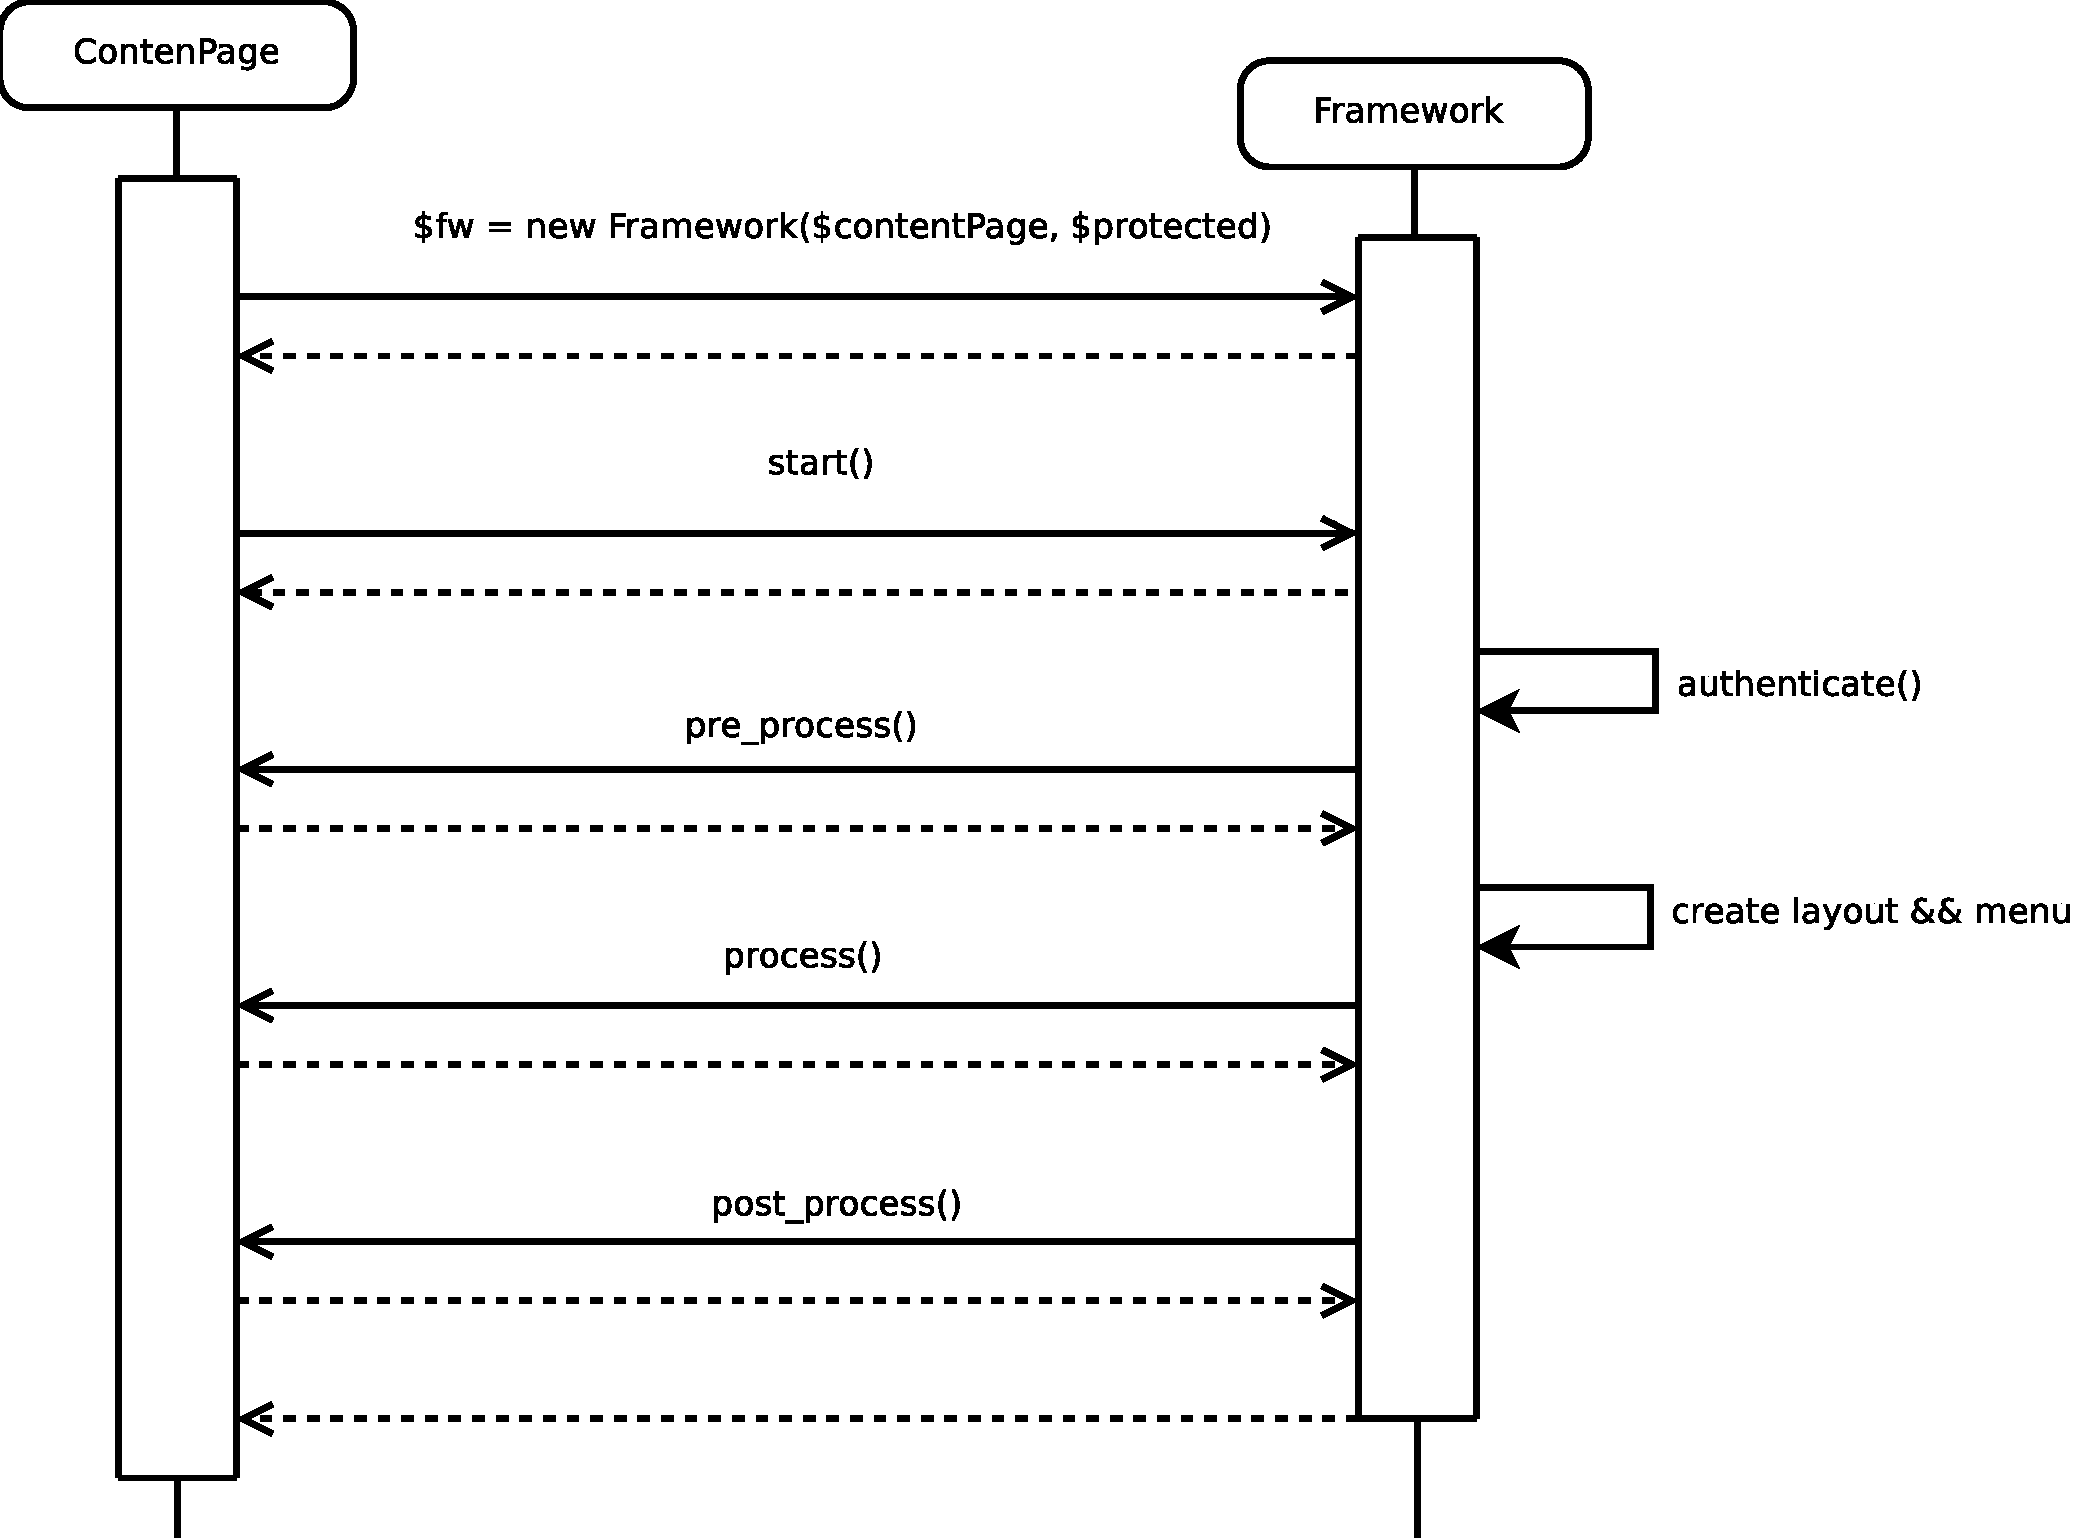
\includegraphics[width=\textwidth]{seq_fw}
	\caption{Sequence diagram of the interaction between the Framework and the ContentPage}
	\end{center}
\end{figure}
\end{document}
